\documentclass[tikz,border=3mm]{standalone}
\usepackage[siunitx]{circuitikz}
\usetikzlibrary{calc,positioning,arrows.meta}

\begin{document}

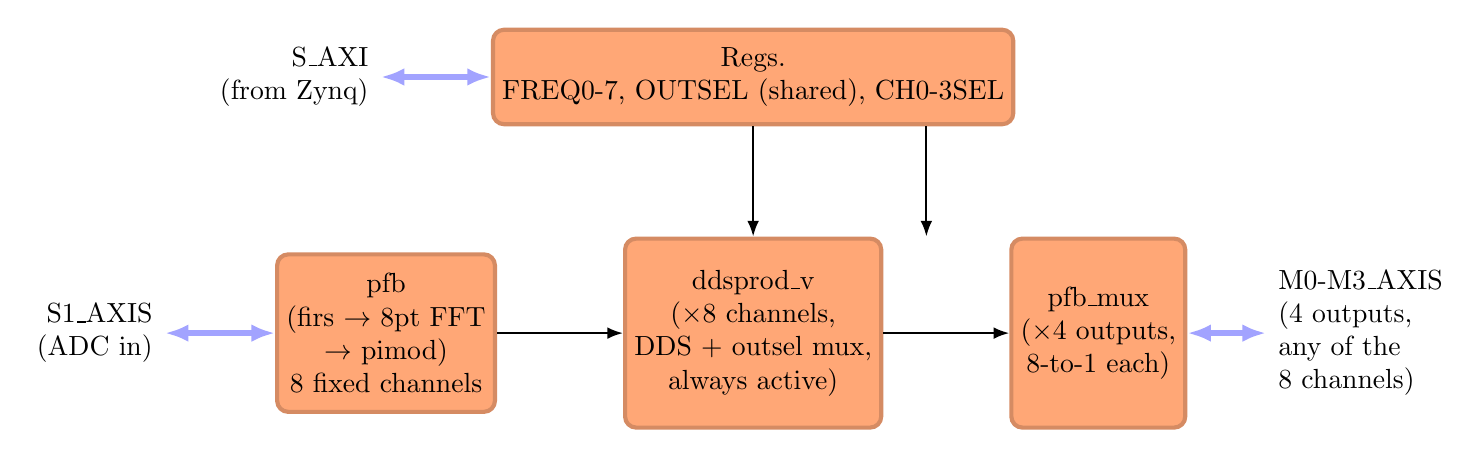
\begin{tikzpicture}
[box/.style={align=center, draw,rounded corners,minimum width=2cm,minimum height=1.2cm,draw={rgb,255:red,213; green,139; blue,99},fill={rgb,255:red,255; green,167; blue,118},line width=1.5pt},
arrow/.style={line width=2.2pt,draw={rgb,255:red,162; green,163; blue,255},{Latex[length=3mm]}-{Latex[length=3mm]}},
single arrow/.style={line width=0.8pt,-{Latex[length=2mm]}},
node distance=0.5cm]

% Channelizer.
\node[box,minimum height=2cm,minimum width=2.4cm] (pfb) {pfb\\(firs $\to$ 8pt FFT\\ $\to$ pimod)\\8 fixed channels};

% Per-channel DDS + outsel mux (always active for all 8 channels).
\node[box,right=1.6cm of pfb,minimum height=2.4cm,minimum width=2.8cm] (dds) {ddsprod\_v\\($\times$8 channels,\\ DDS + outsel mux,\\ always active)};

% Output mux (8-to-1, x4, one per output).
\node[box,right=1.6cm of dds,minimum height=2.4cm,minimum width=2.2cm] (mux) {pfb\_mux\\($\times$4 outputs,\\ 8-to-1 each)};

% Regs.
\coordinate (temp) at ($(dds.north)+(0,1.4)$);
\node[box,anchor=south,minimum width=6.5cm] (regs) at (temp) {Regs.\\FREQ0-7, OUTSEL (shared), CH0-3SEL};

% s1_axis: ADC in.
\draw[arrow] ($(pfb.west)+(-1.4,0)$) coordinate (s1 in) node[anchor=east,align=right] {S1\_AXIS\\(ADC in)} -- (pfb.west);

% s_axi.
\draw[arrow] ($(regs.west)+(-1.4,0)$) node[anchor=east,align=right] {S\_AXI\\(from Zynq)} -- (regs.west);

% pfb -> ddsprod_v.
\draw[single arrow] (pfb.east) -- (dds.west);

% Regs -> ddsprod_v (FREQ0-7, OUTSEL).
\draw[single arrow] (regs.south) -- (regs.south |- dds.north);

% Regs -> pfb_mux (CH0-3SEL).
\coordinate (temp) at ($(regs.south)+(2.2,0)$);
\draw[single arrow] (temp) -- (temp |- mux.north);

% ddsprod_v -> pfb_mux.
\draw[single arrow] (dds.east) -- (mux.west);

% m0-m3_axis.
\draw[arrow] (mux.east) -- ++(1,0) node[anchor=west,align=left] {M0-M3\_AXIS\\(4 outputs,\\ any of the\\ 8 channels)};

\end{tikzpicture}

\end{document}
